% vim: set spell spelllang=en tw=100 et sw=4 sts=4 :

\documentclass{llncs}

\usepackage{microtype}                 % typographic perfection
\usepackage{complexity}                % \P, \NP etc
\usepackage{tikz}                      % For pretty pictures
\usepackage{amsmath}                   % \operatorname
\usepackage{amssymb}                   % \triangledown
\usepackage{hyperref}                  % clicky links
\usepackage{cleveref}                  % no need to type Figure etc
\usepackage[ruled,vlined]{algorithm2e} % algorithms (after cleverref!)
\usepackage{cite}                      % automatically sort mass cites
\usepackage[bottom]{footmisc}          % fix footnote + bottom figure on same page

\usetikzlibrary{arrows, shadows, calc, positioning, decorations, decorations.pathreplacing,
    patterns, matrix, shapes, backgrounds}

% lncs style
\crefname{algocf}{Algorithm}{Algorithms}
\Crefname{algocf}{Algorithm}{Algorithms}
\crefname{figure}{Fig.}{Figs.}
\Crefname{figure}{Fig.}{Figs.}
\crefname{table}{Table}{Tables}
\Crefname{table}{Table}{Tables}
\crefname{proposition}{Proposition}{Propositions}
\Crefname{proposition}{Proposition}{Propositions}

% pretty colours
\definecolor{uofgsandstone}{rgb}{0.321569, 0.278431, 0.231373}
\definecolor{chromayellowgreen}{rgb}{0.882353, 0.984314, 0.788235}
\definecolor{chromagreen}{rgb}{0.564706, 0.933333, 0.564706}
\definecolor{chromateal}{rgb}{0, 0.501961, 0.501961}
\definecolor{chromanavy}{rgb}{0, 0, 0.501961}

\newcommand{\lineref}[1]{line~\ref{#1}}
\newcommand{\twolinesref}[2]{lines~\ref{#1} and~\ref{#2}}

\newcommand*\samethanks[1][\value{footnote}]{\footnotemark[#1]}

\newcommand{\modularproduct}{\operatorname{\triangledown}}

\title{Clique and Constraint Models for Maximum Common (Connected) Subgraph Problems}

\author{Ciaran McCreesh\thanks{This work was supported by the Engineering and Physical Sciences
    Research Council [grant number EP/K503058/1]}\inst{1} \and Samba Ndojh Ndiaye\thanks{This work
was supported by the ANR project SoLStiCe (ANR-13-BS02-0002-01)}\inst{2} \and Patrick
Prosser\inst{1} \and Christine Solnon\samethanks[2] \inst{3}}
\institute{University of Glasgow, Glasgow, Scotland \and
Universit\'e Lyon 1, LIRIS, UMR5205, F-69621, France  \and INSA-Lyon, LIRIS, UMR5205, F-69621, France}

\begin{document}

\maketitle

\begin{abstract}
    The maximum common subgraph problem is to find the largest subgraph common to two given graphs.
    This problem can be solved either by constraint-based search, or by reduction to the maximum
    clique problem. We evaluate these two models using modern algorithms, and see that the best
    choice depends mainly upon whether the graphs have labelled edges. We also study a variant of
    this problem where the subgraph is required to be connected. We introduce a filtering algorithm
    for this property and show that it may be combined with a restricted branching technique for the
    constraint-based approach. We show how to implement a similar branching technique in
    clique-inspired algorithms.  Finally, we experimentally compare approaches for the connected
    version, and see again that the best choice depends on whether graphs have labels.
\end{abstract}

\section{Introduction}

\begin{figure}[b] % first page if possible
    \centering
    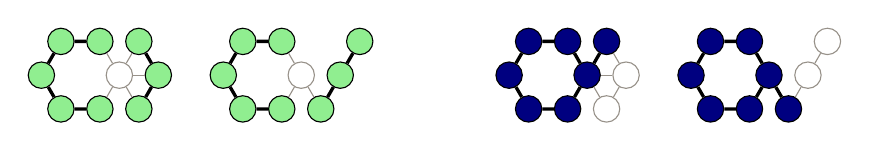
\begin{tikzpicture}[scale=0.33]%{{{
        \begin{scope}[rotate=90]
            \node[draw, circle, fill=chromagreen, inner sep=0.5pt, font=\normalsize] (M1) at (90:1.5) {\phantom{0}};
            \node[draw, circle, fill=chromagreen, inner sep=0.5pt, font=\normalsize] (M2) at (150:1.5) {\phantom{0}};
            \node[draw, circle, fill=chromagreen, inner sep=0.5pt, font=\normalsize] (M3) at (30:1.5) {\phantom{0}};
            \node[draw, circle, fill=chromagreen, inner sep=0.5pt, font=\normalsize] (M4) at (210:1.5) {\phantom{0}};
            \node[draw, circle, fill=chromagreen, inner sep=0.5pt, font=\normalsize] (M5) at (330:1.5) {\phantom{0}};
            \node[draw, circle, draw=uofgsandstone!60, fill=white, inner sep=0.5pt, font=\normalsize] (M6) at (270:1.5) {\phantom{0}};
            \node[draw, circle, fill=chromagreen, inner sep=0.5pt, font=\normalsize] (M7) at ($(210:1.5) + (M6)$) {\phantom{0}};
            \node[draw, circle, fill=chromagreen, inner sep=0.5pt, font=\normalsize] (M8) at ($(330:1.5) + (M6)$) {\phantom{0}};
            \node[draw, circle, fill=chromagreen, inner sep=0.5pt, font=\normalsize] (M9) at ($(270:1.5) + (M6)$) {\phantom{0}};

            \draw [very thick] (M1) -- (M2);
            \draw [very thick] (M2) -- (M4);
            \draw [very thick] (M3) -- (M5);
            \draw [color=uofgsandstone!60] (M4) -- (M6);
            \draw [color=uofgsandstone!60] (M5) -- (M6);
            \draw [very thick] (M3) -- (M1);
            \draw [color=uofgsandstone!60] (M6) -- (M7);
            \draw [color=uofgsandstone!60] (M6) -- (M8);
            \draw [color=uofgsandstone!60] (M6) -- (M9);
            \draw [very thick] (M7) -- (M9);
            \draw [very thick] (M8) -- (M9);
        \end{scope}

        \begin{scope}[xshift=7cm, rotate=90]
            \node[draw, circle, fill=chromagreen, inner sep=0.5pt, font=\normalsize] (M1) at (90:1.5) {\phantom{0}};
            \node[draw, circle, fill=chromagreen, inner sep=0.5pt, font=\normalsize] (M2) at (150:1.5) {\phantom{0}};
            \node[draw, circle, fill=chromagreen, inner sep=0.5pt, font=\normalsize] (M3) at (30:1.5) {\phantom{0}};
            \node[draw, circle, fill=chromagreen, inner sep=0.5pt, font=\normalsize] (M4) at (210:1.5) {\phantom{0}};
            \node[draw, circle, fill=chromagreen, inner sep=0.5pt, font=\normalsize] (M5) at (330:1.5) {\phantom{0}};
            \node[draw, circle, draw=uofgsandstone!60, fill=white, inner sep=0.5pt, font=\normalsize] (M6) at (270:1.5) {\phantom{0}};
            \node[draw, circle, fill=chromagreen, inner sep=0.5pt, font=\normalsize] (M7) at ($(210:1.5) + (M6)$) {\phantom{0}};
            \node[draw, circle, fill=chromagreen, inner sep=0.5pt, font=\normalsize] (M8) at ($(270:1.5) + (M6)$) {\phantom{0}};
            \node[draw, circle, fill=chromagreen, inner sep=0.5pt, font=\normalsize] (M9) at ($(330:1.5) + (M8)$) {\phantom{0}};

            \draw [very thick] (M1) -- (M2);
            \draw [very thick] (M2) -- (M4);
            \draw [very thick] (M3) -- (M5);
            \draw [color=uofgsandstone!60] (M4) -- (M6);
            \draw [color=uofgsandstone!60] (M5) -- (M6);
            \draw [very thick] (M3) -- (M1);
            \draw [color=uofgsandstone!60] (M6) -- (M7);
            \draw [very thick] (M7) -- (M8);
            \draw [very thick] (M8) -- (M9);
        \end{scope}

        \begin{scope}[xshift=18cm, rotate=90]
            \node[draw, circle, fill=chromanavy, inner sep=0.5pt, font=\normalsize] (M1) at (90:1.5) {\phantom{0}};
            \node[draw, circle, fill=chromanavy, inner sep=0.5pt, font=\normalsize] (M2) at (150:1.5) {\phantom{0}};
            \node[draw, circle, fill=chromanavy, inner sep=0.5pt, font=\normalsize] (M3) at (30:1.5) {\phantom{0}};
            \node[draw, circle, fill=chromanavy, inner sep=0.5pt, font=\normalsize] (M4) at (210:1.5) {\phantom{0}};
            \node[draw, circle, fill=chromanavy, inner sep=0.5pt, font=\normalsize] (M5) at (330:1.5) {\phantom{0}};
            \node[draw, circle, fill=chromanavy, inner sep=0.5pt, font=\normalsize] (M6) at (270:1.5) {\phantom{0}};
            \node[draw, circle, draw=uofgsandstone!60, fill=white, inner sep=0.5pt, font=\normalsize] (M7) at ($(210:1.5) + (M6)$) {\phantom{0}};
            \node[draw, circle, fill=chromanavy, inner sep=0.5pt, font=\normalsize] (M8) at ($(330:1.5) + (M6)$) {\phantom{0}};
            \node[draw, circle, draw=uofgsandstone!60, fill=white, inner sep=0.5pt, font=\normalsize] (M9) at ($(270:1.5) + (M6)$) {\phantom{0}};

            \draw [very thick] (M1) -- (M2);
            \draw [very thick] (M2) -- (M4);
            \draw [very thick] (M3) -- (M5);
            \draw [very thick] (M4) -- (M6);
            \draw [very thick] (M5) -- (M6);
            \draw [very thick] (M3) -- (M1);
            \draw [color=uofgsandstone!60] (M6) -- (M7);
            \draw [very thick] (M6) -- (M8);
            \draw [color=uofgsandstone!60] (M6) -- (M9);
            \draw [color=uofgsandstone!60] (M7) -- (M9);
            \draw [color=uofgsandstone!60] (M8) -- (M9);
        \end{scope}

        \begin{scope}[xshift=25cm, rotate=90]
            \node[draw, circle, fill=chromanavy, inner sep=0.5pt, font=\normalsize] (M1) at (90:1.5) {\phantom{0}};
            \node[draw, circle, fill=chromanavy, inner sep=0.5pt, font=\normalsize] (M2) at (150:1.5) {\phantom{0}};
            \node[draw, circle, fill=chromanavy, inner sep=0.5pt, font=\normalsize] (M3) at (30:1.5) {\phantom{0}};
            \node[draw, circle, fill=chromanavy, inner sep=0.5pt, font=\normalsize] (M4) at (210:1.5) {\phantom{0}};
            \node[draw, circle, fill=chromanavy, inner sep=0.5pt, font=\normalsize] (M5) at (330:1.5) {\phantom{0}};
            \node[draw, circle, fill=chromanavy, inner sep=0.5pt, font=\normalsize] (M6) at (270:1.5) {\phantom{0}};
            \node[draw, circle, fill=chromanavy, inner sep=0.5pt, font=\normalsize] (M7) at ($(210:1.5) + (M6)$) {\phantom{0}};
            \node[draw, circle, draw=uofgsandstone!60, fill=white, inner sep=0.5pt, font=\normalsize] (M8) at ($(270:1.5) + (M6)$) {\phantom{0}};
            \node[draw, circle, draw=uofgsandstone!60, fill=white, inner sep=0.5pt, font=\normalsize] (M9) at ($(330:1.5) + (M8)$) {\phantom{0}};

            \draw [very thick] (M1) -- (M2);
            \draw [very thick] (M2) -- (M4);
            \draw [very thick] (M3) -- (M5);
            \draw [very thick] (M4) -- (M6);
            \draw [very thick] (M5) -- (M6);
            \draw [very thick] (M3) -- (M1);
            \draw [very thick] (M6) -- (M7);
            \draw [draw=uofgsandstone!60] (M7) -- (M8);
            \draw [draw=uofgsandstone!60] (M8) -- (M9);
        \end{scope}
\end{tikzpicture}
\caption{A maximum common induced subgraph of the first two graphs has eight vertices, shaded.
However, if we require the common subgraph to be connected, only seven vertices may be
selected---one way to do this is shown in the third and fourth graphs.}\label{figure:mcsexample}
\end{figure}

Maximum common subgraph problems arise in biology and chemistry
\cite{DBLP:journals/jcamd/RaymondW02a,Ehrlich:2011,DAM2014}, in computer vision
\cite{DBLP:journals/jair/CookH94,GBR2013}, in the analysis of source code
\cite{DBLP:journals/tkde/DjokoCH97}, binary programs \cite{DBLP:conf/icics/GaoRS08}, and circuit
designs \cite{DBLP:journals/jair/CookH94}, in character recognition problems \cite{SIWEILU1991617},
and in many other domains \cite{Shasha:2002:AAT:543613.543620}, both directly and as a way of
measuring the similarity or difference between two graphs
\cite{DBLP:journals/prl/Bunke97,DBLP:journals/prl/FernandezV01,KriegeThesis}. We illustrate two
variants of this problem in \cref{figure:mcsexample}---in both cases we are finding an induced
subgraph and maximising the number of vertices selected, but in the second variant the common
subgraph must be connected.

\subsection{Definitions and Notation}

We introduce definitions and algorithms on undirected and unlabelled graphs; the
extension to general graphs is straightforward and is discussed in \cref{extension}. An undirected
graph $G$ is defined by a finite set of vertices $\operatorname{V}(G)$ and a set of undirected edges
$\operatorname{E}(G) \subseteq \operatorname{V}(G) \times \operatorname{V}(G)$, where $(u, v) \in
\operatorname{E}(G) \Rightarrow (v, u) \in \operatorname{E}(G)$. The neighbourhood of
a vertex $v$, written $\operatorname{N}(G, v)$, is the set of vertices to which it is adjacent, so
$\operatorname{N}(G, v) = \{ u \in \operatorname{V}(G) : (u, v) \in \operatorname{E}(G) \}$.
Given a graph $G$, two vertices $v_s, v_e \in \operatorname{V}(G)$ are connected by a path in $G$ if
there exists a sequence of vertices $(v_0, v_1, \ldots, v_k)$ such that $v_0 = v_s$, $v_k = v_e$,
and each pair of successive vertices is connected by an edge, i.e.\ $\forall i\in \{1 \ldots k \},
(v_{i-1}, v_i) \in \operatorname{E}(G)$. A graph $G$ is \emph{connected} if every distinct pair
of vertices is connected by a path.

The \emph{subgraph} of a graph $G$ \emph{induced by} a set $H \subseteq \operatorname{V}(G)$,
written $G[H]$, is the graph with vertex set $H$, and with every edge in $G$ which has both
endpoints in $G$, i.e.\ $\operatorname{E}(G[H]) = \operatorname{E}(G) \cap (\operatorname{V}(H) \times
\operatorname{V}(H))$. We will consider only subgraphs which are induced by some set. It is also
possible to permit removing edges which are not incident to removed vertices, thus leading to
partial subgraphs---we do not consider this possibility in this paper, although everything we
discuss may be extended to the partial case \cite{DBLP:conf/mco/VismaraV08,DBLP:conf/cp/NdiayeS11}.

A graph $G$ is \emph{isomorphic} to another graph $H$ if there exists a bijective function $f :
\operatorname{V}(G) \rightarrow \operatorname{V}(H)$ which preserves edges and non-edges, i.e.\
$\forall (u, v) \in \operatorname{V}(G) \times \operatorname{V}(G), (u, v) \in \operatorname{E}(G)
\Leftrightarrow (f(u),f(v)) \in \operatorname{E}(H)$.  A \emph{common subgraph} of two graphs $G$
and $H$ is a graph isomorphic to subgraphs of both $G$ and $H$. A \emph{common connected subgraph} is a
common subgraph which is connected.  A \emph{Maximum Common Subgraph}, or MCS (resp. \emph{Maximum
Common Connected Subgraph}, or MCCS) is a common subgraph (resp.\ common connected subgraph) which has
a maximum number of vertices.

\subsection{Overview}

In \cref{existing}, we review existing approaches for solving the MCS problem, with a specific focus
on Constraint Programming (CP)-based techniques, and on reductions of the problem to finding a
maximum clique in an association graph.

Previous experimental evaluations have used simple maximum clique algorithms, or even enumeration
algorithms---for example, Vismara and Valery \cite{DBLP:conf/mco/VismaraV08} compare a modified form
of the Bron-Kerbosch maximal clique enumeration algorithm \cite{Bron:1973:AFC:362342.362367} with a
CP optimisation approach. Our experience suggests that a modern maximum clique algorithm could give
many orders of magnitude improvement, due to a strong bound function which prunes the search space.
Therefore, in \cref{eval1}, we re-evaluate the clique-based approach using a modern algorithm, and
we show that it outperforms CP on labelled graphs, and that it is competitive with CP on unlabelled
graphs, contradicting earlier conclusions.

Then, in \cref{mccs}, we consider the MCCS problem. For the CP approach, we may add a global
connectedness constraint to the model. Alternatively, we may use a special branching rule
\cite{DBLP:conf/mco/VismaraV08} to grow connected subgraphs only. These two techniques may be
combined, and we experimentally show that the best results are in fact obtained when combining them.
When solving the MCCS problem with a clique-based approach, neither technique seems directly viable
with an association graph encoding.  However, we show that it is possible to adapt the combined
branching and bounding rule used by modern clique algorithms to maintain connectedness during
search.  We compare the clique-based approach with the best CP variant for MCCS, and we show that it
outperforms CP on labelled graphs, whereas it is outperformed by CP on unlabelled graphs.

\section{Existing Complete Approaches for MCS}\label{existing}

There are two main approaches for solving MCS. The first approach (described in \cref{CP}) is based
on CP, whilst the second (described in \cref{clique}) is based on a reformulation of MCS into a
maximum clique problem. Both approaches are described for undirected, unlabelled graphs; their
extension to richer graphs is discussed in \cref{extension}.  Other approaches have been tried,
mixed integer programming \cite{DBLP:journals/anor/PivaS12} and heuristics
\cite{DBLP:journals/jcisd/EnglertK15}; SAT encodings seem to struggle even for subgraph isomorphism
\cite{UpcomingIJCAIPaper}.

\subsection{Constraint Programming Models for MCS} \label{CP}

McGregor \cite{McGreg82} proposed a branch and bound algorithm: each branch of the search tree
corresponds to the matching of two vertices, and a bounding function evaluates the number of
vertices that still may be matched so that the current branch is pruned as soon as this bound
becomes lower than the size of the largest known common subgraph. CP approaches may be viewed as
enhancements of this branch and bound algorithm.

Vismara and Valery  \cite{DBLP:conf/mco/VismaraV08} introduced the first explicit CP model. Given
two graphs $G$ and $H$, this model associates a variable $x_v$ with every vertex $v$ of $G$, and the
domain of this variable contains all vertices of $H$, plus an additional value $\bot$: variable
$x_v$ is assigned to $\bot$ if vertex $v$ is not matched to any vertex of $H$; otherwise $x_v$ is
assigned to the vertex of $H$ to which it is matched. Edge constraints are introduced in order to
ensure that variable assignments preserve edges and non-edges between matched vertices, i.e.\ $\forall u, v \in
\operatorname{V}(G), (x_u = \bot) \vee (x_v = \bot) \vee ((u, v) \in \operatorname{E}(G)
\Leftrightarrow (x_u, x_v) \in \operatorname{E}(H))$.  Difference constraints are introduced in
order to ensure that each vertex of $H$ is assigned to at most one variable, i.e.\ $\forall u, v \in
\operatorname{V}(G)~\textnormal{distinct,}~ (x_u = \bot) \vee (x_v = \bot) \vee (x_u \neq x_v)$.

This CP model was improved by Ndiaye and Solnon \cite{DBLP:conf/cp/NdiayeS11} by replacing binary
difference constraints with a soft global allDifferent constraint which maximizes the number of
$x_u$ variables that are assigned to values different from $\bot$, while ensuring they are all
different when they are not assigned to $\bot$. They find that the combination ``MAC+Bound'' (resp.
``FC+Bound'') obtains the best results on labelled (resp. unlabelled) graphs and outperforms the
two previous approaches. The combination ``MAC+Bound'' maintains arc consistency~\cite{sabi94} of
edge constraints, whereas the combination ``FC+Bound'' simply performs forward-checking on these
constraints. In both combinations, the ``Bound'' filtering checks whether it is possible to assign
distinct values to enough $x_u$ variables to surpass the best cost found so far---it is a weaker
version of GAC(\emph{softAllDiff}) \cite{peti01} which computes the maximum number of variables that
can be assigned distinct values.

\subsection{Reformulation of MCS to a Maximum Clique Problem}\label{clique}

An alternative approach to MCS is to reduce the problem to finding a maximum clique in an
association graph \cite{LeviG,bala86,dura99,DBLP:journals/jcamd/RaymondW02a}.
An association graph (or compatibility graph, or weak modular product) of two graphs $G$ and $H$ is
an undirected graph $G \modularproduct H$ with vertex set $\operatorname{V}(G \modularproduct H) =
\{ (v, v') \in \operatorname{V}(G) \times \operatorname{V}(H) : (v, v) \in \operatorname{E}(G)
\Leftrightarrow (v', v') \in \operatorname{E}(H)\}$---to avoid confusing vertices of $G \modularproduct
H$ with vertices of the two original graphs, we call vertices of $G \modularproduct H$
\emph{matching nodes}, as each vertex $(u, u')$ of $G \modularproduct H$ denotes the matching of $u$
with $u'$. The edges of $G \modularproduct H$ connect matching nodes which denote compatible
assignments, so two matching nodes $(u, u')$ and  $(v, v')$ are adjacent if $u \neq v$ and $u' \neq
v'$, and if they preserve both edges and non-edges, so $(u, v) \in \operatorname{E}(G)
\Leftrightarrow (u', v') \in \operatorname{E}(H)$. We illustrate this in \cref{figure:association}.

\begin{figure}[tb]
    \centering
    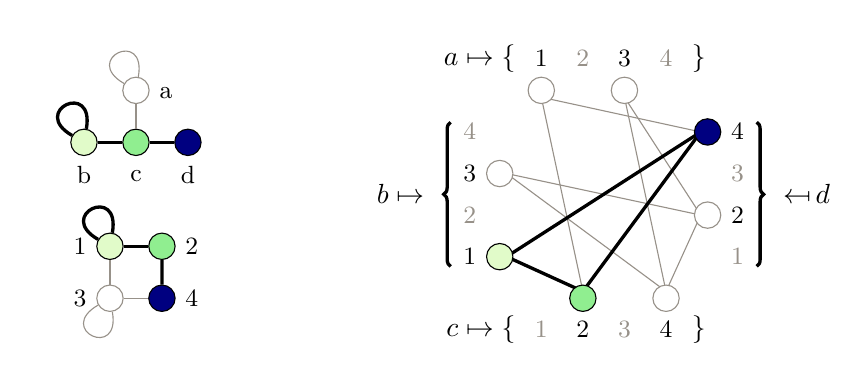
\begin{tikzpicture}[scale=0.33]%{{{
        \begin{scope}
            \node[draw, circle, fill=white, draw=uofgsandstone!60, inner sep=0.5pt, font=\normalsize] (Ma) at (2, 8) {\phantom{0}};
            \node[draw, circle, fill=chromayellowgreen, inner sep=0.5pt, font=\normalsize] (Mb) at (0, 6) {\phantom{0}};
            \node[draw, circle, fill=chromagreen, inner sep=0.5pt, font=\normalsize] (Mc) at (2, 6) {\phantom{0}};
            \node[draw, circle, fill=chromanavy, inner sep=0.5pt, font=\normalsize] (Md) at (4, 6) {\phantom{0}};

            \node [right = 0 of Ma, font=\small] { \vphantom{0}a };
            \node [below = 0 of Mb, font=\small] { \vphantom{0}b };
            \node [below = 0 of Mc, font=\small] { \vphantom{0}c };
            \node [below = 0 of Md, font=\small] { \vphantom{0}d };

            \draw [very thick] (Mb) -- (Mc);
            \draw [very thick] (Mc) -- (Md);
            \draw [color=uofgsandstone!60] (Ma) -- (Mc);
            \draw [color=uofgsandstone!60] (Ma) to [out=150, in=80, looseness=8] (Ma);
            \draw [very thick] (Mb) to [out=150, in=80, looseness=8] (Mb);
        \end{scope}

        \begin{scope}
            \node[draw, circle, fill=chromayellowgreen, inner sep=0.5pt, font=\normalsize] (M1) at (1, 2) {\phantom{0}};
            \node[draw, circle, fill=chromagreen, inner sep=0.5pt, font=\normalsize] (M2) at (3, 2) {\phantom{0}};
            \node[draw, circle, fill=white, draw=uofgsandstone!60, inner sep=0.5pt, font=\normalsize] (M3) at (1, 0) {\phantom{0}};
            \node[draw, circle, fill=chromanavy, inner sep=0.5pt, font=\normalsize] (M4) at (3, 0) {\phantom{0}};

            \node [left = 0 of M1, font=\small] { \vphantom{0}1 };
            \node [right = 0 of M2, font=\small] { \vphantom{0}2 };
            \node [left = 0 of M3, font=\small] { \vphantom{0}3 };
            \node [right = 0 of M4, font=\small] { \vphantom{0}4 };

            \draw [very thick] (M1) -- (M2);
            \draw [very thick] (M2) -- (M4);
            \draw [color=uofgsandstone!60] (M3) -- (M4);
            \draw [color=uofgsandstone!60] (M1) -- (M3);

            \draw [color=uofgsandstone!60] (M3) to [out=280, in=210, looseness=8] (M3);
            \draw [very thick] (M1) to [out=150, in=80, looseness=8] (M1);
        \end{scope}

        \begin{scope}[xshift=15cm, yshift=-1cm]
            \node[draw, circle, fill=white, draw=uofgsandstone!60, inner sep=0.5pt, font=\normalsize] (Ma1) at (2.6, 9) {\phantom{0}};
            \node[draw, circle, fill=white, draw=white, inner sep=0.5pt, font=\normalsize] (Ma2) at (4.2, 9) {\phantom{0}};
            \node[draw, circle, fill=white, draw=uofgsandstone!60, inner sep=0.5pt, font=\normalsize] (Ma3) at (5.8, 9) {\phantom{0}};
            \node[draw, circle, fill=white, draw=white, inner sep=0.5pt, font=\normalsize] (Ma4) at (7.4, 9) {\phantom{0}};
            \node (La1) [above = 0 of Ma1, font=\small] { \vphantom{0}1 };
            \node (La2) [above = 0 of Ma2, font=\small, color=uofgsandstone!60] { \vphantom{0}2 };
            \node (La3) [above = 0 of Ma3, font=\small] { \vphantom{0}3 };
            \node (La4) [above = 0 of Ma4, font=\small, color=uofgsandstone!60] { \vphantom{0}4 };

            \node [left=0 of La1] { $a \mapsto \{$ };
            \node [right=0 of La4] { $\}$ };

            \node[draw, circle, fill=chromayellowgreen, inner sep=0.5pt, font=\normalsize] (Mb1) at (1, 2.6) {\phantom{0}};
            \node[draw, circle, fill=white, draw=white, inner sep=0.5pt, font=\normalsize] (Mb2) at (1, 4.2) {\phantom{0}};
            \node[draw, circle, fill=white, draw=uofgsandstone!60, inner sep=0.5pt, font=\normalsize] (Mb3) at (1, 5.8) {\phantom{0}};
            \node[draw, circle, fill=white, draw=white, inner sep=0.5pt, font=\normalsize] (Mb4) at (1, 7.4) {\phantom{0}};
            \node [left = 0 of Mb1, font=\small] { \vphantom{0}1 };
            \node [left = 0 of Mb2, font=\small, color=uofgsandstone!60] { \vphantom{0}2 };
            \node [left = 0 of Mb3, font=\small] { \vphantom{0}3 };
            \node [left = 0 of Mb4, font=\small, color=uofgsandstone!60] { \vphantom{0}4 };

            \draw [decorate, decoration={brace, raise=0.5cm}, very thick] (Mb1.south west) -- (Mb4.north west)
            node [midway, left=0.7cm] { $b \mapsto$ };

            \node[draw, circle, fill=white, draw=white, inner sep=0.5pt, font=\normalsize] (Mc1) at (2.6, 1) {\phantom{0}};
            \node[draw, circle, fill=chromagreen, inner sep=0.5pt, font=\normalsize] (Mc2) at (4.2, 1) {\phantom{0}};
            \node[draw, circle, fill=white, draw=white, inner sep=0.5pt, font=\normalsize] (Mc3) at (5.8, 1) {\phantom{0}};
            \node[draw, circle, fill=white, draw=uofgsandstone!60, inner sep=0.5pt, font=\normalsize] (Mc4) at (7.4, 1) {\phantom{0}};
            \node (Lc1) [below = 0 of Mc1, font=\small, color=uofgsandstone!60] { \vphantom{0}1 };
            \node (Lc2) [below = 0 of Mc2, font=\small] { \vphantom{0}2 };
            \node (Lc3) [below = 0 of Mc3, font=\small, color=uofgsandstone!60] { \vphantom{0}3 };
            \node (Lc4) [below = 0 of Mc4, font=\small] { \vphantom{0}4 };

            \node [left=0 of Lc1] { $c \mapsto \{$ };
            \node [right=0 of Lc4] { $\}$ };

            \node[draw, circle, fill=white, draw=white, inner sep=0.5pt, font=\normalsize] (Md1) at (9, 2.6) {\phantom{0}};
            \node[draw, circle, fill=white, draw=uofgsandstone!60, inner sep=0.5pt, font=\normalsize] (Md2) at (9, 4.2) {\phantom{0}};
            \node[draw, circle, fill=white, draw=white, inner sep=0.5pt, font=\normalsize] (Md3) at (9, 5.8) {\phantom{0}};
            \node[draw, circle, fill=chromanavy, inner sep=0.5pt, font=\normalsize] (Md4) at (9, 7.4) {\phantom{0}};
            \node [right = 0 of Md1, font=\small, color=uofgsandstone!60] { \vphantom{0}1 };
            \node [right = 0 of Md2, font=\small] { \vphantom{0}2 };
            \node [right = 0 of Md3, font=\small, color=uofgsandstone!60] { \vphantom{0}3 };
            \node [right = 0 of Md4, font=\small] { \vphantom{0}4 };

            \draw [decorate, decoration={brace, raise=0.5cm}, very thick] (Md4.north east) -- (Md1.south east)
            node [midway, right=0.7cm] { $\reflectbox{\ensuremath{\mapsto}}\, d$ };

            \begin{scope}[on background layer]
                \draw [draw=uofgsandstone!60] ($(Ma1.south)!0.5!(Ma1)$) -- ($(Md4.west)!0.5!(Md4)$);
                \draw [draw=uofgsandstone!60] ($(Ma1.south)!0.5!(Ma1)$) -- ($(Mc2.north)!0.5!(Mc2)$);
                \draw [draw=uofgsandstone!60] ($(Ma3.south)!0.5!(Ma3)$) -- ($(Mc4.north)!0.5!(Mc4)$);
                \draw [draw=uofgsandstone!60] ($(Mb3.east)!0.5!(Mb3)$) -- ($(Mc4.north)!0.5!(Mc4)$);
                \draw [draw=uofgsandstone!60] ($(Md2.west)!0.5!(Md2)$) -- ($(Mc4.north)!0.5!(Mc4)$);
                \draw [draw=uofgsandstone!60] ($(Md2.west)!0.5!(Md2)$) -- ($(Ma3.south)!0.5!(Ma3)$);
                \draw [draw=uofgsandstone!60] ($(Md2.west)!0.5!(Md2)$) -- ($(Mb3.east)!0.5!(Mb3)$);
                \draw [very thick] ($(Mb1.east)!0.5!(Mb1)$) -- ($(Mc2.north)!0.5!(Mc2)$);
                \draw [very thick] ($(Mb1.east)!0.5!(Mb1)$) -- ($(Md4.west)!0.5!(Md4)$);
                \draw [very thick] ($(Mc2.north)!0.5!(Mc2)$) -- ($(Md4.west)!0.5!(Md4)$);
        \end{scope}
        \end{scope}

    \end{tikzpicture}

    \caption{A maximum common induced subgraph between the two graphs on the left has three
        vertices---one solution is highlighted. On the right, the association graph encoding: the
        highlighted clique of size three shows the same solution. The ``missing'' vertices
        correspond to assignments which are impossible due to the presence or absence of
        loops.}\label{figure:association}
\end{figure}

A \emph{clique} is a subgraph whose vertices are all pairwise adjacent. A clique is \emph{maximal}
if it is not strictly included in any other clique, and it is \emph{maximum} if it is a largest
clique of a given graph, with respect to the number of vertices.  A clique in an association graph
corresponds to a set of compatible matchings. Therefore, such a clique corresponds to a common
subgraph, and a maximum clique of $G \modularproduct H$ is an MCS of $G$ and $H$.  It follows that
any method able to find a maximum clique in a graph can be used to solve the MCS problem.

Note that the association graph is a partial subgraph of the microstructure
\cite{DBLP:conf/aaai/Jegou93a} associated with the CP model of  Vismara and Valery
\cite{DBLP:conf/mco/VismaraV08}: the microstructure has more matching nodes than the association
graph because it has a matching node $(u,\bot)$ for each vertex $u$ of $G$. Each clique of size
$\left|\operatorname{V}(G)\right|$ in the microstructure corresponds to a common subgraph, the size
of which is defined by the number of matching nodes that do not contain $\bot$.

\subsection{Extension to Labelled or Directed Graphs}\label{extension}

In some applications, labels may be associated with vertices or edges. We denote $\lambda(u)$ and
$\lambda((u, v))$ the label of a vertex $u$ and an edge $(u, v)$, respectively. Where graphs are
labelled, any isomorphism $f$ must additionally preserve labels, so we require $\lambda(f(v)) =
\lambda(v)$ for any vertex $v$, and $\lambda((f(u), f(v))) = \lambda((u, v))$ for any edge $(u, v)$.
This kind of label compatibility constraint is handled in a straightforward way in both CP and
clique-based approaches to MCS.  For CP, we restrict the domain of every variable $x_u$ to vertices
with compatible labels, and ensure that edge labels are preserved in edge constraints.
For clique-based approaches, label compatibility is handled through the definition of the
association graph, by restricting the set of matching nodes to pairs of vertices with compatible
labels, and the set of matching edges to pairs of edges with compatible labels.

The extension of MCS algorithms to directed graphs, where isomorphisms must preserve directed edges,
is similarly straightforward.

Labels and directed edges usually simplify the solution process, both for CP and clique-based
approaches: vertex labels reduce domain sizes for CP, and the number of matching nodes in
association graphs; edge labels tighten edge constraints for CP, and make the association graph
sparser for clique-based approaches. It is worth noting that edge constraints do not help CP
approaches to do more filtering so long as $\bot$ remains in variable domains: every pair of
variables $(x_i, x_j)$ having  $\bot \in D(x_j)$ is arc consistent,
since $\bot$ is a support for any value $u \in D(x_i)$. However, as soon as $\bot$ is removed from
domains (i.e.\ when the number of variables assigned to $\bot$ has reached the best known bound on
the size of the MCS), maintaining arc consistency may filter values, and then tighter constraints
increase the opportunities for filtering.

\section{Re-Evaluating the Clique Model for MCS}\label{eval1}

Previous experimental evaluations of the association graph model have used either maximal clique
enumeration algorithms \cite{DBLP:journals/tcs/Koch01,DBLP:conf/mco/VismaraV08} (even when the
maximisation problem was being considered), or very simple maximum clique algorithms
\cite{DBLP:conf/sspr/BunkeFGSV02,DBLP:journals/jgaa/ConteFV07}, and so their conclusions may now be
overly pessimistic. Thus we re-evaluate the approach using a modern maximum clique algorithm.
Association graphs are dense, even if the input is sparse, so we will using (the single-threaded,
bit-parallel version of) the maximum clique solver by McCreesh and Prosser
\cite{DBLP:journals/topc/McCreeshP15}, which implements Prosser's
\cite{DBLP:journals/algorithms/Prosser12} ``MCSa1'' variant of a series of algorithms due to Tomita
\textit{et al.}\
\cite{DBLP:conf/dmtcs/TomitaS03,DBLP:journals/jgo/TomitaK07,DBLP:conf/walcom/TomitaSHTW10}, using a
bitset encoding due to San Segundo \textit{et al.}\
\cite{DBLP:journals/cor/SegundoRJ11,DBLP:journals/ol/SegundoMRH13}. We compare this to the
``FC+Bound'' and ``MAC+Bound'' (simply referred to as FC and MAC) CP implementations of Ndiaye and
Solnon \cite{DBLP:conf/cp/NdiayeS11}, using smallest domain first for variable ordering, and a value
ordering which prefers vertices of most similar degree.  We perform our experiments on machines with
Intel Xeon E5-2640 v2 CPUs and 64GBytes RAM; software was compiled using GCC 4.9, and a timeout of
one hour was used.

We consider a randomly generated database
\cite{DBLP:journals/prl/SantoFSV03,DBLP:journals/jgaa/ConteFV07} commonly used for benchmarking
maximum common subgraph problems.  The dataset contains different classes of graphs: randomly
connected graphs with different densities; 2D, 3D, and 4D regular and irregular meshes; regular
bounded valence graphs, and irregular bounded valence graphs.  For each pair of graphs, there are 3
different labellings such that the number of different labels is equal to 33\%, 50\% or 75\% of the
number of vertices. In this paper, we report experiments with unlabelled graphs (labels are
ignored), and with 33\% labellings (the problem becomes very easy with larger numbers of labels).
For unlabelled graphs, we select the 27,500 graph pairs where the number of vertices in each graph
is no more than 35; for labelled graphs, which we find less computationally challenging, we select
all 81,400 graph pairs, to include graphs with up to 100 vertices.

\begin{figure}[tb]
    \centering
    \includegraphics{gen-graph-unconnected-cumulative.pdf}
    \vspace*{1em}

    \centering
    \includegraphics{gen-graph-unconnected-heatmap.pdf}
    \caption{The cumulative number of MCS instances solved in under a certain time: on the top, 33\%
        labelled graphs, and then unlabelled and undirected graphs. On the bottom, an
        instance-by-instance comparison of the clique model with the best CP model, with 33\%
        labelled graphs (with MAC) on the left, and unlabelled and undirected graphs (with FC) on
    the right.} \label{figure:unconnected-cumulative}
\end{figure}

The two plots on the top of \cref{figure:unconnected-cumulative} display the cumulative number of
instances solved with respect to time.  When graphs are labelled, the clique-based approach clearly
outperforms either CP model, and MAC has a slight advantage over FC. (Recall that edge labels
    decrease the density of the association graph, which is typically very beneficial for clique
algorithms, but do not help CP until $\bot$ is removed from domains.) For unlabelled graphs, the
three approaches are broadly comparable, and ultimately FC beats MAC, which beats the clique
approach. The bottom row gives a per-instance comparison of the best CP approach with the clique
approach: the heatmaps are similar to scatter plots, but due to the large number of instances, we
colour each point according to the density of solutions around that point. For labelled graphs, the
clique approach comes close to dominating MAC on non-trivial instances (which suggests that there is
unlikely to be scope for per-instance algorithm selection here). For unlabelled graphs, there is
still a broad correlation between the runtimes; the clique approach rarely wins by more than one
order of magnitude, but is sometimes much worse.

A closer inspection of the data suggests that the different randomness models used to generate
instances have little effect on the runtimes for either approach. However, the relative size of the
solution matters, particularly for the clique algorithm: if the solution is large (i.e.\ the two
input graphs are very similar), the clique approach finds nearly every labelled instance trivial.

\section{Finding Maximum Common Connected Subgraphs}\label{mccs}

In many applications, the common subgraph must satisfy some additional constraints. This
is usually handled in a straightforward way in CP, by branching rules and/or constraint
propagation. In clique-based approaches, some constraints may be handled by modifying the
definition of the association graph---for example, constraints on pairs of vertices that may be
matched are handled by removing inconsistent pairs from $\operatorname{V}(G \modularproduct H)$.
However, more global constraints cannot be handled by modifying the definition of the association
graph.

In this paper, we focus on the connectedness constraint, which occurs in many applications
\cite{DBLP:journals/tcs/Koch01,DBLP:journals/jcamd/RaymondW02a,DBLP:conf/mco/VismaraV08,Ehrlich:2011}.
Adding the connectedness requirement makes certain special cases solvable in polynomial time,
including outerplanar graphs of bounded degree \cite{DBLP:journals/algorithms/AkutsuT13} and trees
\cite{droschinsky_et_al:LIPIcs:2016:xxxx}, but the general case remains \NP-hard. As illustrated in
\cref{figure:mcsexample}, the MCCS cannot be deduced from the MCS: we need to ensure connectedness
during search. In \cref{mccs-cp}, we show that in CP this may be done in two different ways that
may be combined, and we show in \cref{mccs-cp-eval} that the best results are obtained when
combining them. In \cref{mccs-clique}, we introduce a new way for ensuring connectedness in a
clique-based approach. Finally, we compare CP and our clique-based approach in \cref{mccs-eval}.

For MCCS we consider only undirected graphs (and so we treat directed edges in the inputs as being
undirected). For directed graphs, there is more than one notion of connectivity, and it is not clear
which should be selected---the approaches we consider extend easily to weakly connected directed
graphs, but not to the strongly connected case (for which we know of no applications).

\subsection{Ensuring Connectedness in CP}\label{mccs-cp}

Vismara and Valery \cite{DBLP:conf/mco/VismaraV08} implement the connectedness constraint by using a
branching rule which selects the next variable to be assigned. Let $A$ be the
set of variables already assigned to values different from $\bot$. The next variable to be assigned
is chosen within the set of unassigned variables which are the neighbour of at least one vertex of
$A$.  When this set is empty, all remaining unassigned variables are assigned to
$\bot$. We illustrate this in \cref{figure:restricted}.

\begin{figure}[tb]
    \newcounter{stepcounter}
    \centering
    \begin{tikzpicture}[scale=0.33]%{{{
        \begin{scope}
            \node[draw, circle, fill=white, inner sep=0.5pt, font=\normalsize] (Ma) at (0, 4) {\phantom{0}};
            \node[draw, circle, fill=white, inner sep=0.5pt, font=\normalsize] (Mb) at (0, 2) {\phantom{0}};
            \node[draw, circle, fill=white, inner sep=0.5pt, font=\normalsize] (Mc) at (2, 2) {\phantom{0}};
            \node[draw, circle, fill=white, inner sep=0.5pt, font=\normalsize] (Md) at (0, 0) {\phantom{0}};
            \node[draw, circle, fill=white, inner sep=0.5pt, font=\normalsize] (Me) at (2, 0) {\phantom{0}};

            \node [left = 0 of Ma, font=\small] { \vphantom{0}a };
            \node [left = 0 of Mb, font=\small] { \vphantom{0}b };
            \node [right = 0 of Mc, font=\small] { \vphantom{0}c };
            \node [left = 0 of Md, font=\small] { \vphantom{0}d };
            \node [right = 0 of Me, font=\small] { \vphantom{0}e };

            \draw [draw=uofgsandstone!60] (Ma) -- (Mb);
            \draw [draw=uofgsandstone!60] (Ma) -- (Mc);
            \draw [draw=uofgsandstone!60] (Mb) -- (Mc);
            \draw [draw=uofgsandstone!60] (Mb) -- (Md);
            \draw [draw=uofgsandstone!60] (Mc) -- (Me);

            \node[draw, circle, fill=white, inner sep=0.5pt, font=\normalsize] (M1) at (5.6, 4) {\phantom{0}};
            \node[draw, circle, fill=white, inner sep=0.5pt, font=\normalsize] (M2) at (7.6, 4) {\phantom{0}};
            \node[draw, circle, fill=white, inner sep=0.5pt, font=\normalsize] (M3) at (5.6, 2) {\phantom{0}};
            \node[draw, circle, fill=white, inner sep=0.5pt, font=\normalsize] (M4) at (7.6, 2) {\phantom{0}};
            \node[draw, circle, fill=white, inner sep=0.5pt, font=\normalsize] (M5) at (5.6, 0) {\phantom{0}};

            \node [left = 0 of M1, font=\small] { \vphantom{0}1 };
            \node [right = 0 of M2, font=\small] { \vphantom{0}2 };
            \node [left = 0 of M3, font=\small] { \vphantom{0}3 };
            \node [right = 0 of M4, font=\small] { \vphantom{0}4 };
            \node [left = 0 of M5, font=\small] { \vphantom{0}5 };

            \draw [color=uofgsandstone!60] (M1) -- (M2);
            \draw [color=uofgsandstone!60] (M1) -- (M3);
            \draw [color=uofgsandstone!60] (M2) -- (M4);
            \draw [color=uofgsandstone!60] (M3) -- (M4);

            \node [anchor=base, yshift=-2.2cm] at ($(Ma)!0.5!(M2)$) {
                \stepcounter{stepcounter}\roman{stepcounter}) Initial problem };
        \end{scope}

        \begin{scope}[xshift=12.8cm]
            \node[draw, circle, fill=chromayellowgreen, inner sep=0.5pt, font=\normalsize] (Ma) at (0, 4) {\phantom{0}};
            \node[draw, circle, fill=white, inner sep=0.5pt, font=\normalsize] (Mb) at (0, 2) {\phantom{0}};
            \node[draw, circle, fill=white, inner sep=0.5pt, font=\normalsize] (Mc) at (2, 2) {\phantom{0}};
            \node[draw, dotted, circle, fill=white, inner sep=0.5pt, font=\normalsize] (Md) at (0, 0) {\phantom{0}};
            \node[draw, dotted, circle, fill=white, inner sep=0.5pt, font=\normalsize] (Me) at (2, 0) {\phantom{0}};

            \node [left = 0 of Ma, font=\small] { \vphantom{0}a };
            \node [left = 0 of Mb, font=\small] { \vphantom{0}b };
            \node [right = 0 of Mc, font=\small] { \vphantom{0}c };
            \node [left = 0 of Md, font=\small] { \vphantom{0}d };
            \node [right = 0 of Me, font=\small] { \vphantom{0}e };

            \draw [draw=uofgsandstone!60] (Ma) -- (Mb);
            \draw [draw=uofgsandstone!60] (Ma) -- (Mc);
            \draw [draw=uofgsandstone!60] (Mb) -- (Mc);
            \draw [dotted] (Mb) -- (Md);
            \draw [dotted] (Mc) -- (Me);

            \node[draw, circle, fill=chromayellowgreen, inner sep=0.5pt, font=\normalsize] (M1) at (5.6, 4) {\phantom{0}};
            \node[draw, circle, fill=white, inner sep=0.5pt, font=\normalsize] (M2) at (7.6, 4) {\phantom{0}};
            \node[draw, circle, fill=white, inner sep=0.5pt, font=\normalsize] (M3) at (5.6, 2) {\phantom{0}};
            \node[draw, circle, fill=white, inner sep=0.5pt, font=\normalsize] (M4) at (7.6, 2) {\phantom{0}};
            \node[draw, circle, fill=white, inner sep=0.5pt, font=\normalsize] (M5) at (5.6, 0) {\phantom{0}};

            \node [left = 0 of M1, font=\small] { \vphantom{0}1 };
            \node [right = 0 of M2, font=\small] { \vphantom{0}2 };
            \node [left = 0 of M3, font=\small] { \vphantom{0}3 };
            \node [right = 0 of M4, font=\small] { \vphantom{0}4 };
            \node [left = 0 of M5, font=\small] { \vphantom{0}5 };

            \draw [color=uofgsandstone!60] (M1) -- (M2);
            \draw [color=uofgsandstone!60] (M1) -- (M3);
            \draw [color=uofgsandstone!60] (M2) -- (M4);
            \draw [color=uofgsandstone!60] (M3) -- (M4);

            \node [anchor=base, yshift=-2.2cm] at ($(Ma)!0.5!(M2)$) {
                \stepcounter{stepcounter}\roman{stepcounter}) Trying $a \mapsto 1$ };
        \end{scope}

        \begin{scope}[xshift=25.6cm]
            \node[draw, circle, fill=chromayellowgreen, inner sep=0.5pt, font=\normalsize] (Ma) at (0, 4) {\phantom{0}};
            \node[draw, circle, fill=chromagreen, inner sep=0.5pt, font=\normalsize] (Mb) at (0, 2) {\phantom{0}};
            \node[draw, circle, fill=white, draw=uofgsandstone!60, inner sep=0.5pt, font=\normalsize] (Mc) at (2, 2) {\phantom{0}};
            \node[draw, circle, fill=white, inner sep=0.5pt, font=\normalsize] (Md) at (0, 0) {\phantom{0}};
            \node[draw, dotted, circle, fill=white, inner sep=0.5pt, font=\normalsize] (Me) at (2, 0) {\phantom{0}};

            \node [left = 0 of Ma, font=\small] { \vphantom{0}a };
            \node [left = 0 of Mb, font=\small] { \vphantom{0}b };
            \node [right = 0 of Mc, font=\small] { \vphantom{0}c };
            \node [left = 0 of Md, font=\small] { \vphantom{0}d };
            \node [right = 0 of Me, font=\small] { \vphantom{0}e };

            \draw [very thick] (Ma) -- (Mb);
            \draw [color=uofgsandstone!60] (Ma) -- (Mc);
            \draw [color=uofgsandstone!60] (Mb) -- (Mc);
            \draw [color=uofgsandstone!60] (Mb) -- (Md);
            \draw [color=uofgsandstone!60] (Mc) -- (Me);

            \node[draw, circle, fill=chromayellowgreen, inner sep=0.5pt, font=\normalsize] (M1) at (5.6, 4) {\phantom{0}};
            \node[draw, circle, fill=chromagreen, inner sep=0.5pt, font=\normalsize] (M2) at (7.6, 4) {\phantom{0}};
            \node[draw, circle, fill=white, inner sep=0.5pt, font=\normalsize] (M3) at (5.6, 2) {\phantom{0}};
            \node[draw, circle, fill=white, inner sep=0.5pt, font=\normalsize] (M4) at (7.6, 2) {\phantom{0}};
            \node[draw, circle, fill=white, inner sep=0.5pt, font=\normalsize] (M5) at (5.6, 0) {\phantom{0}};

            \node [left = 0 of M1, font=\small] { \vphantom{0}1 };
            \node [right = 0 of M2, font=\small] { \vphantom{0}2 };
            \node [left = 0 of M3, font=\small] { \vphantom{0}3 };
            \node [right = 0 of M4, font=\small] { \vphantom{0}4 };
            \node [left = 0 of M5, font=\small] { \vphantom{0}5 };

            \draw [very thick] (M1) -- (M2);
            \draw [color=uofgsandstone!60] (M1) -- (M3);
            \draw [color=uofgsandstone!60] (M2) -- (M4);
            \draw [color=uofgsandstone!60] (M3) -- (M4);

            \node [anchor=base, yshift=-2.2cm] at ($(Ma)!0.5!(M2)$) {
                \stepcounter{stepcounter}\roman{stepcounter}) Trying $b \mapsto 2$ };
        \end{scope}

        \begin{scope}[yshift=-9cm]
            \node[draw, circle, fill=chromayellowgreen, inner sep=0.5pt, font=\normalsize] (Ma) at (0, 4) {\phantom{0}};
            \node[draw, circle, fill=chromagreen, inner sep=0.5pt, font=\normalsize] (Mb) at (0, 2) {\phantom{0}};
            \node[draw, circle, fill=white, draw=uofgsandstone!60, inner sep=0.5pt, font=\normalsize] (Mc) at (2, 2) {\phantom{0}};
            \node[draw, circle, fill=chromanavy, inner sep=0.5pt, font=\normalsize] (Md) at (0, 0) {\phantom{0}};
            \node[draw, dotted, circle, fill=white, inner sep=0.5pt, font=\normalsize] (Me) at (2, 0) {\phantom{0}};

            \node [left = 0 of Ma, font=\small] { \vphantom{0}a };
            \node [left = 0 of Mb, font=\small] { \vphantom{0}b };
            \node [right = 0 of Mc, font=\small] { \vphantom{0}c };
            \node [left = 0 of Md, font=\small] { \vphantom{0}d };
            \node [right = 0 of Me, font=\small] { \vphantom{0}e };

            \draw [very thick] (Ma) -- (Mb);
            \draw [color=uofgsandstone!60] (Ma) -- (Mc);
            \draw [color=uofgsandstone!60] (Mb) -- (Mc);
            \draw [very thick] (Mb) -- (Md);
            \draw [color=uofgsandstone!60] (Mc) -- (Me);

            \node[draw, circle, fill=chromayellowgreen, inner sep=0.5pt, font=\normalsize] (M1) at (5.6, 4) {\phantom{0}};
            \node[draw, circle, fill=chromagreen, inner sep=0.5pt, font=\normalsize] (M2) at (7.6, 4) {\phantom{0}};
            \node[draw, circle, fill=white, inner sep=0.5pt, font=\normalsize] (M3) at (5.6, 2) {\phantom{0}};
            \node[draw, circle, fill=chromanavy, inner sep=0.5pt, font=\normalsize] (M4) at (7.6, 2) {\phantom{0}};
            \node[draw, circle, fill=white, inner sep=0.5pt, font=\normalsize] (M5) at (5.6, 0) {\phantom{0}};

            \node [left = 0 of M1, font=\small] { \vphantom{0}1 };
            \node [right = 0 of M2, font=\small] { \vphantom{0}2 };
            \node [left = 0 of M3, font=\small] { \vphantom{0}3 };
            \node [right = 0 of M4, font=\small] { \vphantom{0}4 };
            \node [left = 0 of M5, font=\small] { \vphantom{0}5 };

            \draw [very thick] (M1) -- (M2);
            \draw [color=uofgsandstone!60] (M1) -- (M3);
            \draw [very thick] (M2) -- (M4);
            \draw [color=uofgsandstone!60] (M3) -- (M4);

            \node [anchor=base, yshift=-2.2cm] at ($(Ma)!0.5!(M2)$) {
                \stepcounter{stepcounter}\roman{stepcounter}) Trying $d \mapsto 4$ };
        \end{scope}

        \begin{scope}[xshift=12.8cm, yshift=-9cm]
            \node[draw, circle, fill=chromayellowgreen, inner sep=0.5pt, font=\normalsize] (Ma) at (0, 4) {\phantom{0}};
            \node[draw, circle, fill=chromagreen, inner sep=0.5pt, font=\normalsize] (Mb) at (0, 2) {\phantom{0}};
            \node[draw, circle, fill=white, draw=uofgsandstone!60, inner sep=0.5pt, font=\normalsize] (Mc) at (2, 2) {\phantom{0}};
            \node[draw, circle, fill=chromanavy, inner sep=0.5pt, font=\normalsize] (Md) at (0, 0) {\phantom{0}};
            \node[draw, circle, fill=white, draw=uofgsandstone!60, inner sep=0.5pt, font=\normalsize] (Me) at (2, 0) {\phantom{0}};

            \node [left = 0 of Ma, font=\small] { \vphantom{0}a };
            \node [left = 0 of Mb, font=\small] { \vphantom{0}b };
            \node [right = 0 of Mc, font=\small] { \vphantom{0}c };
            \node [left = 0 of Md, font=\small] { \vphantom{0}d };
            \node [right = 0 of Me, font=\small] { \vphantom{0}e };

            \draw [very thick] (Ma) -- (Mb);
            \draw [color=uofgsandstone!60] (Ma) -- (Mc);
            \draw [color=uofgsandstone!60] (Mb) -- (Mc);
            \draw [very thick] (Mb) -- (Md);
            \draw [color=uofgsandstone!60] (Mc) -- (Me);

            \node[draw, circle, fill=chromayellowgreen, inner sep=0.5pt, font=\normalsize] (M1) at (5.6, 4) {\phantom{0}};
            \node[draw, circle, fill=chromagreen, inner sep=0.5pt, font=\normalsize] (M2) at (7.6, 4) {\phantom{0}};
            \node[draw, circle, fill=white, inner sep=0.5pt, font=\normalsize] (M3) at (5.6, 2) {\phantom{0}};
            \node[draw, circle, fill=chromanavy, inner sep=0.5pt, font=\normalsize] (M4) at (7.6, 2) {\phantom{0}};
            \node[draw, circle, fill=white, inner sep=0.5pt, font=\normalsize] (M5) at (5.6, 0) {\phantom{0}};

            \node [left = 0 of M1, font=\small] { \vphantom{0}1 };
            \node [right = 0 of M2, font=\small] { \vphantom{0}2 };
            \node [left = 0 of M3, font=\small] { \vphantom{0}3 };
            \node [right = 0 of M4, font=\small] { \vphantom{0}4 };
            \node [left = 0 of M5, font=\small] { \vphantom{0}5 };

            \draw [very thick] (M1) -- (M2);
            \draw [color=uofgsandstone!60] (M1) -- (M3);
            \draw [very thick] (M2) -- (M4);
            \draw [color=uofgsandstone!60] (M3) -- (M4);

            \node [anchor=base, yshift=-2.2cm] at ($(Ma)!0.5!(M2)$) {
                \stepcounter{stepcounter}\roman{stepcounter}) $e \mapsto \bot$ is forced };
        \end{scope}
    \end{tikzpicture}

    \caption{Suppose we are looking for a connected common subgraph, using the graph on the left
        for variables and the graph on the right (which has an isolated vertex) for values. We
        initially consider $a \mapsto 1$. Our restricted branching rule requires us to select either variable
        $b$ or variable $c$ subsequently, not $d$ or $e$. We try $b \mapsto 2$, which adds $d$
        to the branchable variables, and forces $c \mapsto \bot$. We may now only branch on $d$, and
        we try $d \mapsto 4$. Now the only remaining variable is unbranchable, and so $e = \bot$ is forced, even
        though $5$ remains in its domain and does not violate any constraints.}\label{figure:restricted}
\end{figure}

A more traditional CP approach would be to express connectedness as a conventional constraint. For
example, CP(Graph) \cite{DBLP:conf/cp/DoomsDD05} introduces graph domain variables and enforces
connectivity via the \emph{reachable} constraint, ensuring that there is a path from a specified
vertex to a specified set of vertices. One such constraint could be posted for each of the vertices
in the graph, encoding the transitive closure of the graph. Brown et al.\ \cite{Brown:2005}
explored the use of constraint programming in the generation of connected graphs with specified
degree sequences.  Two constraints were combined: the graphical constraint (a backtrackable
implementation of the Havel-Hakimi algorithm), and a connectivity constraint implemented using sets
of vertices, where vertex sets $A$ and $B$ are combined when there exists a pair of vertices $v \in
A$ and $w \in B$ and an edge $(v,w) \in E$. Residual degree counts are maintained on components and
vertices to enforce graphicality and connectivity. Prosser and Unsworth
\cite{DBLP:conf/ecai/ProsserU06} proposed a connectivity constraint for connected graph generation
where decision variables are edges (the search process accepts and rejects edges). The constraint
employed depth first search to maintain the set of tree edges and back edges, associating path
counters on these edges. The counters were then used to detect the existence of cut-edges and
protects these by forcing edges.

In all these previous works, the goal was to ensure that a given set of vertices is connected. For
MCCS, the problem is slightly different: we have to ensure that the number of connected vertices
that may be matched (in both graphs) is greater than the size of the largest common subgraph
previously found. Therefore, we introduce a new filtering algorithm to ensure connectedness
consistency for MCCS.  Let us consider two graphs $G$ and $H$, and let $D$ be the current domains
(we suppose that $D(x_u)$ is a singleton when $x_u$ is assigned). Let $S$ and $T$ be the sets of
vertices of $G$ and $H$ respectively which may belong to the common subgraph, i.e.\ $S=\{ u\in
\operatorname{V}(G) : D(x_u)\neq\{\bot\}\}$, and $T = \cup_{u\in \operatorname{V}(G)} D(x_u)
\setminus \{ \bot \}$. Connectedness consistency ensures that both $G[S]$ and $H[T]$ are
connected graphs.

Connectedness consistency is ensured only once a first variable has been assigned, rather than at
the root of search. Let $x_u$ be the first assigned variable, and $v$ the value
assigned to $x_u$. To ensure connectedness consistency, we perform a traversal of $G$ (resp.\ $H$),
starting from $u$ (resp.\ $v$), and we initialize $S$ (resp.\ $T$) with all visited vertices. Then,
for each vertex $v\in \operatorname{V}(G) \setminus S$, we set $x_v$ to $\bot$, and for each $w
\in \operatorname{V}(H) \setminus T$, we remove $w$ from all domains to which it belongs.

During search, each time a variable is assigned to $\bot$, we remove the corresponding vertex
from $S$ and perform a new traversal of $G[S]$ starting from the initial vertex $u$. For each vertex
$w\in S$ that is not visited by the traversal, we remove $w$ from $S$ and assign $x_w$ to $\bot$.
Also, each time a value is removed from a domain so that this value no longer belongs to any domain,
we remove it from $T$, and perform a new traversal of $H[T]$ starting from the initial vertex $v$.
For each vertex $w$ that is not visited by the traversal, we remove $w$ from $T$, and remove $w$
from all domains to which it belongs.

Finally, the two approaches for ensuring connectedness (branching and filtering) are complementary
and may be combined: at each step of the search, we select the next variable to be assigned within
the neighbors of $A$, and each time a vertex of $H$ is removed from a domain we filter domains to
ensure connectedness consistency. In the example in \cref{figure:restricted}, after the first
assignment, filtering alone would remove $5$ from every domain but would allow branching on any
remaining variable, whilst branching alone would force the next variable to be either $b$ or $c$ but
would not immediately eliminate $5$ from the domains of $d$ and $e$.

\begin{figure}[tb]
    \centering
    \includegraphics{gen-graph-connected-cumulative-cp.pdf}

    \vspace*{0.5em}
    \centering
    \includegraphics{gen-graph-connected-cp.pdf}
    \caption{On top, the cumulative number of MCCS instances solved in under a certain time using
        different CP techniques, for 33\% labelled (left) and unlabelled undirected (right) graphs.
    Below, instance-by-instance comparisons.}
        \label{figure:connected-cp}
\end{figure}

\subsection{Experimental Comparison of CP Connectedness Techniques}\label{mccs-cp-eval}

\Cref{figure:connected-cp} compares the three approaches for ensuring connectedness in CP: by
branching (Branch), by filtering (Filter), or by combining branching and filtering (Both). We show
only results using the best variant for each class---that is, MAC for labelled graphs, and FC for
unlabelled graphs (the other results are very similar).  On labelled graphs, we see many instances
which are solved very quickly by branching but not at all by filtering, and vice versa.  However,
combining both is rarely much worse than just doing one or the other, and is often much better, even
if on average it is slightly slower.  On unlabelled graphs, the three variants have rather similar
performance.

\subsection{Ensuring Connectedness in a Clique-Based Approach}\label{mccs-clique}

It is not possible to determine connectedness from a raw association graph. However, we can take a
maximum clique algorithm and mimic the CP branching strategy if we have access to the underlying
graphs and can determine the ``meaning'' of the association graph vertices.

Most modern maximum clique algorithms for dense graphs use some variation of greedy graph colouring
as a bound---the underlying observation is that each vertex in a clique must be given a different
colour in a colouring, so if we can colour a subset of vertices using $k$ colours then a maximum
clique in this subset has at most $k$ vertices. However, the colouring is also used as a branching
heuristic: vertices are selected in reverse order from their colour classes in turn, starting with the
last colour class created. Because of this coupling of branching and the bound (which is important
in practice because it mimics a ``smallest domain first'' branching heuristic if colour classes are
viewed as variables, without requiring a new bound to be calculated for every iteration
\cite{DBLP:conf/cp/McCreeshP14}), if we were to select only a subset of vertices for branching at
each stage inside a clique algorithm, we would lose completeness. Thus we must adapt the bound in a
non-trivial way to take into account restricted branching.

\begin{algorithm}[tb] \DontPrintSemicolon
\nl $\FuncSty{associationMCCIS}$ :: (Graph $G_1$, Graph $G_2$) $\rightarrow$ Map \;
\nl \Begin{
    \nl $\KwSty{global} ~ \mathit{incumbent} \gets \emptyset$ \label{incumbent} \;
    \nl $G \gets G_1 \modularproduct G_2$ \label{buildassoc} \;
    \nl $\FuncSty{search}(G, \emptyset, \emptyset, \operatorname{V}(G))$ \label{firstsearch} \;
    \nl $\KwSty{return} ~ \mathit{incumbent}$ \;
}
\nl $\FuncSty{search}$ :: (Graph $G$, Set $\mathit{solution}$, Set $\mathit{connected}$, Set $\mathit{remaining}$) \;
\nl \Begin{
    \nl $\mathit{colourClasses} \gets \FuncSty{concatenate}($ \label{makecolours} \;
    $\hspace*{2em}\FuncSty{colour}(G, \mathit{remaining} \setminus \mathit{connected}),\,\FuncSty{colour}(G, \mathit{remaining} \cap \mathit{connected}))$ \;
    \nl \While{$\FuncSty{length}(\mathit{colourClasses}) > 0$\label{outerloop}}{
        \nl \ForEach{$v \in \FuncSty{last}(\mathit{colourClasses}) \textnormal{~in reverse order}$\label{innerloop}}{
            \nl \lIf{$|\mathit{solution}| + \FuncSty{length}(\mathit{colourClasses}) \leq
            |\mathit{incumbent}|$}{\KwSty{return}\label{bound}}
            \nl \lIf{$v \notin \mathit{connected} ~ \KwSty{and} ~ \mathit{solution} \ne
            \emptyset$}{\KwSty{return} \label{acceptbranchable}}
            \nl $\mathit{solution}' \gets \mathit{solution} \cup \{ v \} \label{addv} \label{addvtosolution} $\;
            \nl \lIf{$|\mathit{solution}'| > |\mathit{incumbent}|$}{$\mathit{incumbent} \gets
            \mathit{solution}'$ \label{newincumbent}}
            \nl $\mathit{connected}' \gets \mathit{connected} \cup \{ w \in G : \FuncSty{first}(w)
            \in \operatorname{N}(G, \FuncSty{first}(v)) \}$ \label{addtobranchable} \;
            \nl $\mathit{remaining}' \gets \mathit{remaining} \cap \operatorname{N}(G, v)$ \label{filterremaining} \;
            \nl \lIf{$\mathit{remaining}' \neq \emptyset$}{$\FuncSty{search}(G, \mathit{solution}',
            \mathit{connected}', \mathit{remaining}')$\label{recursesearch}}
         }
         \nl $\FuncSty{removeLast}(\mathit{colourClasses})$ \;
     }
}
\nl $\FuncSty{colour}$ :: (Graph $G$, Set $\mathit{uncoloured}$) $\rightarrow$ List of List of Vertex \;
\nl \Begin{
    \nl $\KwSty{return}$ a greedy colouring of the vertices in $\mathit{uncoloured}$,
    using the procedure of San Segundo et al.\ \cite{DBLP:journals/cor/SegundoRJ11} with a static
    degree order from $G$ and $k_{\mathit{min}} = 0$. \;
}
\caption{An algorithm for a maximum common connected induced subgraph isomorphism via an association graph.}
\label{algorithm:mccis}
\end{algorithm}

In \cref{algorithm:mccis} we present a novel clique-inspired algorithm which finds a maximum common
connected induced subgraph via an association graph. If the additional branching
restrictions are removed, the core of the algorithm is the same as the ``MCSa1'' clique algorithm
used in the previous section (and we refer the reader to the previously cited works for
implementation details on how to use bitsets and other data structures to implement the colouring
stage with very low constant factors). The way we extend this algorithm for connectedness differs
considerably from that of Koch \cite{DBLP:journals/tcs/Koch01} and Vismara and Valery
\cite{DBLP:conf/mco/VismaraV08}: these earlier approaches worked by classifying labels in the
association graph based upon whether a common vertex is shared, and then constructing cliques with
particular edge properties---this is harder to integrate with a strong bound function.

Our algorithm begins by building the association graph (\lineref{buildassoc}). The main part of the algorithm
then works by building up candidate cliques in the $\mathit{solution}$ variable, by recursive calls
to the $\mathit{search}$ procedure---starting from the empty set (\lineref{firstsearch}), each
recursive subcall adds one vertex to $\mathit{solution}$ (\lineref{addv}) in such a way that
$\mathit{solution}$ is always a clique which corresponds to a connected common subgraph. The
$\mathit{remaining}$ set contains the set of vertices which are adjacent to every vertex in
$\mathit{solution}$, and which have not yet been accepted or rejected (and so initially it contains
every vertex). The main loops in the $\FuncSty{search}$ procedure
(\twolinesref{outerloop}{innerloop}) have the effect of iterating over each vertex in this set in a
particular order---each vertex $v$ is selected in turn, and then a recursive call is made to
consider the effects of including $v$ in $\mathit{solution}$ (\lineref{recursesearch}), followed by
the next iteration where $v$ is instead rejected. When $v$ is accepted, we add it to the new
$\mathit{solution'}$ (\lineref{addvtosolution}), and create a new $\mathit{remaining'}$ containing
only the vertices in $\mathit{remaining}$ which are adjacent to $v$ (\lineref{filterremaining}).

The $\mathit{connected}$ set contains the set of matching nodes which correspond to
vertices adjacent to an already-accepted vertex in the first input graph---in constraint programming terms, it is the
set of assignments which could be made next which maintain connectedness. (Using only one of the two
input graphs is sufficient for correctness, and has the advantage that the connectedness set
may be determined by a simple lookup into a precomputed array which maps each vertex in
the first input graph to a bitset.) At the top of search, this set is empty, and is not used (our
first vertex selection is special, and does not care about connectedness). At subsequent depths, we
may only accept vertices which are in this set, and if no such vertices remain then we return
immediately (\lineref{acceptbranchable}). When recursing, we extend $\mathit{connected}$ with the
new vertices permitted by our acceptance of the branching $v$ (\lineref{addtobranchable}). Note that
we are assuming that inside the main loops, we encounter every vertex in $\mathit{remaining} \cap
\mathit{connected}$ before any vertex in $\mathit{remaining} \setminus \mathit{connected}$.

As we proceed, we keep track of the best solution we have found so far---this is stored in the
$\mathit{incumbent}$ variable (\twolinesref{incumbent}{newincumbent}). We use the incumbent,
together with a colour bound, to prune portions of the search space which cannot contain a better
solution. The colour bound operates as follows: at each entry to the $\FuncSty{search}$ procedure,
we produce a greedy colouring of the vertices in $\mathit{remaining}$ (\lineref{makecolours},
discussed further below). This greedy colouring gives us a list of colour classes, each of which is
a list of pairwise non-adjacent vertices. The two loops (\twolinesref{outerloop}{innerloop}) then
iterate over each colour class, from last to first, and then over each vertex in that colour class,
again from last to first.  (Rather than actually using a list of lists and removing items, this
process should be implemented using a pair of immutable flat arrays. This technique is described
elsewhere \cite{DBLP:conf/cp/McCreeshP14}, so we do not discuss it here.) Finally, if at any point
the number of remaining colour classes plus the number of vertices currently present in
$\mathit{solution}$ is not strictly greater than the size of the incumbent, then we may backtrack
immediately (\lineref{bound}).

\begin{figure}[tb]
    \newcounter{stepcounter2}
    \centering
    \begin{tikzpicture}[scale=0.33]%{{{
        \matrix (m) [matrix of nodes, column sep=0.5cm] {
            \begin{tikzpicture}[scale=0.33]
                    \node[draw, circle, fill=white, inner sep=0.5pt, font=\normalsize] (Ma) at (0, 4) {\phantom{0}};
                    \node[draw, circle, fill=white, inner sep=0.5pt, font=\normalsize] (Mb) at (2, 4) {\phantom{0}};
                    \node[draw, circle, fill=white, inner sep=0.5pt, font=\normalsize] (Mc) at (0, 2) {\phantom{0}};
                    \node[draw, circle, fill=white, inner sep=0.5pt, font=\normalsize] (Md) at (2, 2) {\phantom{0}};
                    \node[draw, circle, fill=white, inner sep=0.5pt, font=\normalsize] (Me) at (0, 0) {\phantom{0}};
                    \node[draw, circle, fill=white, inner sep=0.5pt, font=\normalsize] (Mf) at (2, 0) {\phantom{0}};

                    \node [left = 0 of Ma, font=\small] { \vphantom{0}a };
                    \node [right = 0 of Mb, font=\small] { \vphantom{0}b };
                    \node [left = 0 of Mc, font=\small] { \vphantom{0}c };
                    \node [right = 0 of Md, font=\small] { \vphantom{0}d };
                    \node [left = 0 of Me, font=\small] { \vphantom{0}e };
                    \node [right = 0 of Mf, font=\small] { \vphantom{0}f };

                    \draw (Ma) -- (Mb);
                    \draw (Ma) -- (Mc);
                    \draw (Ma) -- (Md);
                    \draw (Mc) -- (Md);
                    \draw (Mc) -- (Me);
                    \draw (Md) -- (Mf);

                    \node[draw, circle, fill=white, inner sep=0.5pt, font=\normalsize] (M1) at (6, 4) {\phantom{0}};
                    \node[draw, circle, fill=white, inner sep=0.5pt, font=\normalsize] (M2) at (8, 4) {\phantom{0}};
                    \node[draw, circle, fill=white, inner sep=0.5pt, font=\normalsize] (M3) at (6, 2) {\phantom{0}};
                    \node[draw, circle, fill=white, inner sep=0.5pt, font=\normalsize] (M4) at (8, 2) {\phantom{0}};
                    \node[draw, circle, fill=white, inner sep=0.5pt, font=\normalsize] (M5) at (6, 0) {\phantom{0}};

                    \node [left = 0 of M1, font=\small] { \vphantom{0}1 };
                    \node [right = 0 of M2, font=\small] { \vphantom{0}2 };
                    \node [left = 0 of M3, font=\small] { \vphantom{0}3 };
                    \node [right = 0 of M4, font=\small] { \vphantom{0}4 };
                    \node [left = 0 of M5, font=\small] { \vphantom{0}5 };

                    \draw [color=uofgsandstone!60] (M1) -- (M2);
                    \draw [color=uofgsandstone!60] (M1) -- (M3);
                    \draw [color=uofgsandstone!60] (M2) -- (M4);
                    \draw [color=uofgsandstone!60] (M3) -- (M4);
            \end{tikzpicture}
            &
            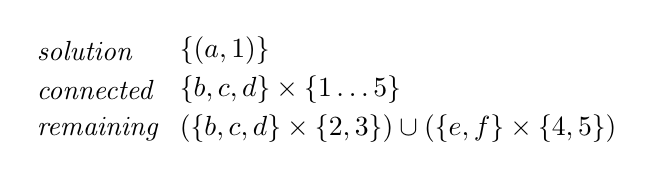
\begin{tikzpicture}[scale=0.33]
                    \node [anchor=west] (Ns) at (0, 3.5) { $\mathit{solution}$ };
                    \node [anchor=west] (Nb) at (0, 2) { $\mathit{connected}$ };
                    \node [anchor=west] (Nr) at (0, 0.5) { $\mathit{remaining}$ };

                    \node [anchor=west] (Vs) at (5.5, 3.5) { $\{ (a, 1) \}$ };
                    \node [anchor=west] (Vb) at (5.5, 2) { $\{ b, c, d \} \times \{1 \ldots 5 \}$ };
                    \node [anchor=west] (Vr) at (5.5, 0.5) { $(\{ b, c, d \} \times \{ 2, 3 \}) \cup (\{ e, f\} \times \{ 4, 5 \})$ };
            \end{tikzpicture}
            \\[0.1cm]
            \stepcounter{stepcounter2}\roman{stepcounter2}) Initial problem &
            \stepcounter{stepcounter2}\roman{stepcounter2}) Search variables after guessing $a \mapsto 1$
            \\[0.2cm]
            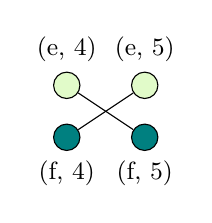
\begin{tikzpicture}[scale=0.33]
                    \node[draw, circle, fill=chromayellowgreen, inner sep=0.5pt, font=\normalsize] (Me4) at (0, 2) {\phantom{0}};
                    \node[draw, circle, fill=chromayellowgreen, inner sep=0.5pt, font=\normalsize] (Me5) at (3, 2) {\phantom{0}};
                    \node[draw, circle, fill=chromateal, inner sep=0.5pt, font=\normalsize] (Mf4) at (0, 0) {\phantom{0}};
                    \node[draw, circle, fill=chromateal, inner sep=0.5pt, font=\normalsize] (Mf5) at (3, 0) {\phantom{0}};

                    \node [above = 0 of Me4, font=\small] { \vphantom{0}(e, 4) };
                    \node [above = 0 of Me5, font=\small] { \vphantom{0}(e, 5) };
                    \node [below = 0 of Mf4, font=\small] { \vphantom{0}(f, 4) };
                    \node [below = 0 of Mf5, font=\small] { \vphantom{0}(f, 5) };

                    \draw (Me4) -- (Mf5);
                    \draw (Me5) -- (Mf4);
            \end{tikzpicture}
            &
            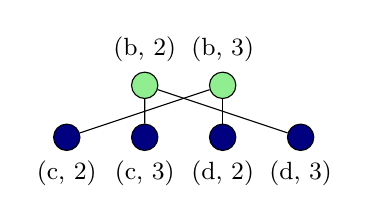
\begin{tikzpicture}[scale=0.33]
                    \node[draw, circle, fill=chromagreen, inner sep=0.5pt, font=\normalsize] (Mb2) at (3, 2) {\phantom{0}};
                    \node[draw, circle, fill=chromagreen, inner sep=0.5pt, font=\normalsize] (Mb3) at (6, 2) {\phantom{0}};
                    \node[draw, circle, fill=chromanavy, inner sep=0.5pt, font=\normalsize] (Mc2) at (0, 0) {\phantom{0}};
                    \node[draw, circle, fill=chromanavy, inner sep=0.5pt, font=\normalsize] (Mc3) at (3, 0) {\phantom{0}};
                    \node[draw, circle, fill=chromanavy, inner sep=0.5pt, font=\normalsize] (Md2) at (6, 0) {\phantom{0}};
                    \node[draw, circle, fill=chromanavy, inner sep=0.5pt, font=\normalsize] (Md3) at (9, 0) {\phantom{0}};

                    \node [above = 0 of Mb2, font=\small] { \vphantom{0}(b, 2) };
                    \node [above = 0 of Mb3, font=\small] { \vphantom{0}(b, 3) };
                    \node [below = 0 of Mc2, font=\small] { \vphantom{0}(c, 2) };
                    \node [below = 0 of Mc3, font=\small] { \vphantom{0}(c, 3) };
                    \node [below = 0 of Md2, font=\small] { \vphantom{0}(d, 2) };
                    \node [below = 0 of Md3, font=\small] { \vphantom{0}(d, 3) };

                    \draw (Mb2) -- (Mc3);
                    \draw (Mb2) -- (Md3);
                    \draw (Mb3) -- (Mc2);
                    \draw (Mb3) -- (Md2);
            \end{tikzpicture}
            \\[0.1cm]
            \stepcounter{stepcounter2}\roman{stepcounter2}) $\mathit{remaining} \setminus
            \mathit{connected}$ &
            \stepcounter{stepcounter2}\roman{stepcounter2}) $\mathit{remaining} \cap
            \mathit{connected}$
            \\
        };
    \end{tikzpicture}\\[0.1cm]\begin{tikzpicture}[scale=0.33]
        \matrix (m) [matrix of nodes] {
            \begin{tikzpicture}[scale=0.33]
                \node[draw, circle, fill=chromayellowgreen, inner sep=0.5pt, font=\normalsize] (Me4) at (0, 0) {\phantom{0}};
                \node[draw, circle, fill=chromayellowgreen, inner sep=0.5pt, font=\normalsize] (Me5) at (3, 0) {\phantom{0}};
                \node[draw, circle, fill=chromateal, inner sep=0.5pt, font=\normalsize] (Mf4) at (6, 0) {\phantom{0}};
                \node[draw, circle, fill=chromateal, inner sep=0.5pt, font=\normalsize] (Mf5) at (9, 0) {\phantom{0}};
                \node[draw, circle, fill=chromagreen, inner sep=0.5pt, font=\normalsize] (Mb2) at (12, 0) {\phantom{0}};
                \node[draw, circle, fill=chromagreen, inner sep=0.5pt, font=\normalsize] (Mb3) at (15, 0) {\phantom{0}};
                \node[draw, circle, fill=chromanavy, inner sep=0.5pt, font=\normalsize] (Mc2) at (18, 0) {\phantom{0}};
                \node[draw, circle, fill=chromanavy, inner sep=0.5pt, font=\normalsize] (Mc3) at (21, 0) {\phantom{0}};
                \node[draw, circle, fill=chromanavy, inner sep=0.5pt, font=\normalsize] (Md2) at (24, 0) {\phantom{0}};
                \node[draw, circle, fill=chromanavy, inner sep=0.5pt, font=\normalsize] (Md3) at (27, 0) {\phantom{0}};

                \node [above = 0 of Me4, font=\small, xshift=-0.5ex] { \vphantom{0}[[(e, 4), };
                \node [above = 0 of Me5, font=\small] { \vphantom{0}(e, 5)], };
                \node [above = 0 of Mf4, font=\small] { \vphantom{0}[(f, 4), };
                \node [above = 0 of Mf5, font=\small] { \vphantom{0}(f, 5)], };
                \node [above = 0 of Mb2, font=\small] { \vphantom{0}[(b, 2), };
                \node [above = 0 of Mb3, font=\small] { \vphantom{0}(b, 3)], };
                \node [above = 0 of Mc2, font=\small] { \vphantom{0}[(c, 2), };
                \node [above = 0 of Mc3, font=\small] { \vphantom{0}(c, 3), };
                \node [above = 0 of Md2, font=\small] { \vphantom{0}(d, 2), };
                \node [above = 0 of Md3, font=\small] { \vphantom{0}(d, 3)]]};
            \end{tikzpicture}
            \\[0.05cm]
            \stepcounter{stepcounter2}\roman{stepcounter2}) The resulting $\mathit{colourClasses}$ variable.
            \\
        };
    \end{tikzpicture}

    \caption{Solving a maximum common connected problem using an association graph. Suppose we
        have already mapped vertex $a$ to vertex $1$, giving the assignments on the right. Now we
        have two subgraphs to colour. We need two colours for $\mathit{remaining} \setminus
        \mathit{connected}$, and we place these two colour classes first in the $\mathit{colourClasses}$
        variable. We can also colour $\mathit{remaining} \cap \mathit{connected}$ using two
        colours, since we cannot simultaneously map $c$ to $2$ and $d$ to $3$, or vice-versa. Thus
        $\mathit{colourClasses}$ becomes a list of four colour classes. This tells us that if we hope to
        extend the current common subgraph by another four vertices, we
        must pick one assignment from each of the four colour classes (which is not actually
        possible, so the bound here gives an overestimate). The algorithm thus guesses $d \mapsto 3$ as its next
assignment, and if that fails, $d \mapsto 2$, and so on; once $b \mapsto 3$ is reached, the bound
decreases by one, and if $f \mapsto 5$ were reached we would stop due to a lack of remaining
connected association nodes. }\label{figure:assocrestricted}
\end{figure}

Finally, we describe the colouring process---an example is shown in \cref{figure:assocrestricted}.
In conventional clique algorithms, a simple greedy sequential colouring is used (possibly with the
help of previous colourings to reduce the computational cost \cite{DBLP:conf/lion/NikolaevBS15}, and
possibly with shortcuts taken for certain vertices \cite{DBLP:journals/cor/SegundoT14}, and possibly
followed by a repair step to improve the colouring \cite{DBLP:conf/walcom/TomitaSHTW10}, or stronger
bounding rules based upon MaxSAT inference
\cite{DBLP:conf/ictai/LiFX13,DBLP:conf/lion/LiJX15,DBLP:journals/cor/SegundoNB15}).  Such colourings
will not give us the required property that vertices in $\mathit{remaining} \cap \mathit{connected}$
come last (so they are selected first by the reverse branching order). Thus we produce two greedy
sequential colourings, first considering the non-branching vertices in $\mathit{remaining} \setminus
\mathit{connected}$, followed by the branching vertices, and concatenate them
(\lineref{makecolours}). This produces a valid colouring, since we do not merge any colour classes
between the two stages, although it may use more colours than a single colouring would.

(What if we did not guarantee that vertices in $\mathit{remaining} \cap \mathit{connected}$ came
last, and just used a conventional colouring with the branching rule?  Suppose we had four vertices
in $\mathit{remaining}$, and produced a colouring $[[v_1, v_2], [v_3], [v_4]]$, and suppose that
extending $\mathit{solution}$ with $\{ v_1, v_3, v_4 \}$ gives an optimal solution. If $v_4$ was not
$\mathit{connected}$ yet, we would not branch on that subtree, and the bound could eliminate
branching on $v_3$ and $v_1$, so we would miss the solution. Thus we cannot simply add the branching
rule without also adapting the combined bound and ordering heuristic.)

Our $\FuncSty{colour}$ procedure is a simple greedy sequential colouring. We use the bit-parallel
algorithm introduced by San Segundo \textit{et al.}\ \cite{DBLP:journals/cor/SegundoRJ11}, with the
$k_{\mathit{min}}$ parameter set to $0$, so we do not describe it here. We use a simple static degree
ordering; other initial vertex orderings have been considered on general clique problems
\cite{DBLP:journals/algorithms/Prosser12,DBLP:conf/lion/SegundoLB14}, and it is possible that
special properties of the association graph could be exploited in this step (for example, it is
always possible to colour the initial association graph using
$\operatorname{min}(\left|\operatorname{V}(G_1)\right|, \left|\operatorname{V}(G_2)\right|)$
colours, but with certain vertex orderings, a greedy sequential colouring will sometimes use
many more colours).

\subsection{Experimental Comparison of the CP and Clique Approaches}\label{mccs-eval}

\begin{figure}[tb]
    \centering
    \includegraphics{gen-graph-connected-cumulative.pdf}
    \vspace*{1em}

    \centering
    \includegraphics{gen-graph-connected-heatmap.pdf}
    \caption{The cumulative number of connected instances solved in under a certain time: on the
        top, 33\% labelled undirected graphs with up to 100 vertices, and then unlabelled
        and undirected graphs with up to 35 vertices. On the bottom, an instance-by-instance
        comparison of the association and CP Both approaches, with 33\% labelled graphs on the
        left, and unlabelled and undirected graphs on the right.} \label{figure:connected-cumulative}
\end{figure}

In \cref{figure:connected-cumulative} we compare the clique-based approach to the connected problem
with the two CP Both approaches. The trend is broadly similar to the unconnected problem: for labelled
graphs, the clique-based approach is the clear winner, but for unlabelled graphs the clique approach
lags somewhat.

The heatmaps show a more detailed picture. As before, in the unlabelled case, the association
approach is almost never more than an order of magnitude better, and is often much worse. In the
labelled case, however, there are now many instances where the CP approach does much better than the
association approach, despite the association approach remaining much better overall.

\section{Conclusion}

Contradicting earlier claims in the literature, we have seen that a modern clique algorithm can
perform competitively for maximum common subgraph problems, particularly when edge labels are
involved. However, the best approaches for these problems is still far behind the state-of-the-art
for subgraph isomorphism, where we can often scale to unlabelled graphs with thousands of vertices.

To start tackling this gap, we believe there is further scope for tailoring clique algorithms for
association graphs, including specialised inference, a bound function which is aware that it is
working on an association graph, and better initial vertex orderings. Treating the first branch
specially may also be beneficial, since the first branch has an unusually large effect on the search
space with association graphs \cite{DBLP:conf/cocoon/SutersAZSSL05}.

For CP models, using a branching rule for connectedness, rather than simply as an ordering heuristic,
is unconventional and does not cleanly fit into the abstractions used by toolkits. However, we saw
that combining conventional filtering and the special branching rule was beneficial.

We looked only at single-threaded versions of these algorithms. Maximum clique algorithms have been
extended for thread-parallel search
\cite{DBLP:journals/algorithms/McCreeshP13,DBLP:journals/jcisd/DepolliKRTJ13,DBLP:journals/cor/SegundoLP16},
and in particular, work stealing strategies designed to eliminate exceptionally hard instances by
forcing diversity at the top of search \cite{DBLP:journals/topc/McCreeshP15} could be beneficial in
eliminating some of the rare cases where the clique algorithm is many orders of magnitude worse than
the CP models. On the CP side, the focus for parallelism has been on decomposition
\cite{DBLP:conf/ictai/MinotNS15}, rather than fully dynamic work stealing---it would be interesting
to compare these approaches.

Finally, we intend to investigate larger and more diverse sets of instances, and other variants of
the problem. We have yet to investigate partial or weighted graphs. Nor have we considered strongly
connected common subgraphs---this would make the branching approach impossible, and filtering would
be much more complicated. From the datasets we selected, there appears to be little scope for
per-instance algorithm selection, but other families of input data could lead to a different
conclusion.

\bibliographystyle{splncs}
\bibliography{paper}

\end{document}

